\section{Further discussion on Computer Algebra}
\label{sec:moretheory}

Bit level circuit variables including primary inputs/outputs can only take value
within $\Z_2$. They can also be written in functions of other variables and constants.
In computer algebra, circuit variable $a$ can be described as a polynomial, that is
$a = f(x_0, x_1, \dots, x_{n-1}) \in {\mathbb{F}}[x]$. Moreover, circuit variable can
have multiple specifications, they can be written in polynomials and included in an
ideal $I = \{f_0, f_1, \dots, f_k\}$. The varieties of this ideal are possible 
assignments of circuit variable. Similarly for $n$ bits world-level circuit 
variables, the varieties are elements from $\Fkk$. Thus it's convenient to use
ideals and varieties to describle circuit variables. \par

\begin{Definition}
({\bf Sum of Ideals}) If I and J are ideals in $k[x_1, \dots, x_n]$, then the 
{\bf sum} of I and J, denoted I + J, is the set
  \begin{equation}
  I + J = \{f + g : f \in I and g \in J\}.
  \end{equation}
Furthermore, if $I = \langle f_1, \dots, f_r\rangle$ and 
$J = \langle g_1, \dots, g_s\rangle$, then 
$I + J = \langle f_1, \dots, f_r, g_1, \dots, g_s\rangle$.
\end{Definition}

\begin{Definition}
({\bf Product of Ideals}) If I and J are ideals in $k[x_1, \dots, x_n]$, then the
{\bf product} of I and J, denoted $I \cdot J$, is defined to be the ideal generated 
by all polynomials $f \cdot g$ where $f \in I$ and $g \in J$. Furthermore, let
$I = \langle f_1, \dots, f_r\rangle$ and $J = \langle g_1, \dots, g_s\rangle$, then
  \begin{equation}
  I \cdot J = \langle f_ig_j : 1 \leq i \leq r, 1 \leq j \leq s\rangle .
  \end{equation}
\end{Definition}

\begin{Definition}
({\bf Quotient of Ideals}) If I and J are ideals in $k[x_1, \dots, x_n]$, then I:J
is the set
  \begin{equation}
  \{f \in k[x_1, \dots, x_n] : fg \in I \forall g \in J\}
  \end{equation}
and is called the {\bf ideal quotient} of I by J.
\end{Definition}

According to definitions above, it's possible to calculate ideal sum, product and 
quotient based on ideal generators. Additionally conclusion about union, 
intersection and complement of varieties can be attained below: \par

\begin{Theorem}
\label{thm:unionintersect}
If I and J are ideals in $k[x_1, \dots, x_n]$, then ${\bf V}(I + J) = {\bf V}(I)
\bigcap {\bf V}(J)$ and ${\bf V}(I \cdot J) = {\bf V}(I) \bigcup {\bf V}(J)$.
\end{Theorem}

\begin{Theorem}
\label{thm:quotient}
Let V and W be varieties in $\Fkk$. Then ${\bf I}(V) : {\bf I}(W) = 
{\bf I}(V - W)$.
\end{Theorem}

For \ref{thm:quotient}, let $V = \Fkk = {\bf V}(\langle vanishing polynomials
\rangle)$, then $V - W$ is the complementary set of variety $W$.\\

Based on these conclusions it's easy to get a circuit variable's specifications
or possible assignments from the other known information.





\section{Sequential circuits and Finite State Machine}
\label{sec:fsm}
{\bf Introduction to Finite State Machine:}\par
{\bf Symbolic Image Computation:}\par
{\bf Implicit State Enumeration:}\par





\section{Experiments using new approach}
\label{sec:exp}

First example is reachable state enumeration of a 2-bit finite state machine.
Breadth-First-Search traversal (mentioned in \ref{sec:fsm}) is adopted.

\begin{Example}
\label{ex:traversal}
Sample circuit is described below with gate-level implement and state transition
graph.
  \begin{figure}[hbt]
    \centerline{\includegraphics[scale=0.3]{./fsm_ckt.png}}
    \caption{Sample circuit}
  \label{fig:fsmckt}
  \end{figure}

  \begin{figure}[hbt]
    \centerline{\includegraphics[scale=0.3]{./fsm_stg.png}}
    \caption{State Transition Graph}
  \label{fig:fsmstg}
  \end{figure}

The following mapping from Boolean operations to Gal\"ois field $\mathbb{F}_2$ 
operations is straightforward. Assuming $a$ and $b$ are both bit-level variables:
\begin{itemize}
  \item $\bar{a} \rightarrow 1 + a$
  \item $a and b \rightarrow ab$
  \item $a or b \rightarrow a + b + ab$
\end{itemize}
Comparing to the quantification approach in \ref{sec:fsm}, using Gr\"obner bases
approach from \ref{sec:theory}. Construct an elimination ideal with following 
polynomials: $f_1: 1 + XNOR(t0, OR(p\cdot q, (1+xi)\cdot(1+p)\cdot(1+q))); 
f_2: 1 + XNOR(t1, OR(xi\cdot(1+p),p\cdot(1+q))); f_3: S - p - q\cdot\alpha; 
f_4: T - t0 - t1\cdot\alpha$ and vanishing polynomials $f_5: p^2 - p; 
f_6: q^2 - q; f_7: t0^2 - t0; f_8: t1^2 - t1; f_9: S^4 - S; f_{10}: xi^2 - xi; 
f_{11}: T^4 - T$, where $S$ and $T$ are 2-bit word representing current state
and next state as defined in $f_3$ and $f_4$, $f_1$ and $f_2$ describe the 
transition relations. At last the initial state should also be included in 
this elimination ideal. For example initial state is $S_3$, then last polynomial
is $f_{12}: S + 1 + \alpha$. According to elimination theorem \ref{thm:elim},
let the lex ordering be $\{all others\} > T$, calculate Gr\"obner basis, the 
result must contain a polynomial with only one variable $T$, which can indicate
the possible assignments of next state. \par

Apply this approach to calculate image in BFS traversal \ref{alg:BFS}.
In this example, $to^i$ and $reached$ are both ideals containing only one
generator, i.e. the polynomial with single variable $T$; universal set is
varieties from ideal $\langle T^4 - T\rangle$. Use \ref{thm:unionintersect} and
\ref{thm:quotient} to complete \ref{alg:BFS}, the final return value is 
polynomial $to^3 = T^4 + T$, which means all states are rechable from state $S_3$.
\end{Example}

The second example shows the application of the new approach on sequential 
arithematic circuits function verification.

\begin{Example}
\label{exp:multiplier}

The following design is Sequential Multiplier with Parallel Output (SMPO),
a Normal Basis multiplier based on Massey-Omura algorithm. Inputs and outputs
are all 5-bit word taking value from ${\mathbb F}_{2^5}$. After loading operands
 A and B, setting all output latches to 0 and running for 6 iterations, the 
output should be $R = A\cdot B$ (mod $x^5 + x^2 + 1$).
  \begin{figure}[hbt]
    \centerline{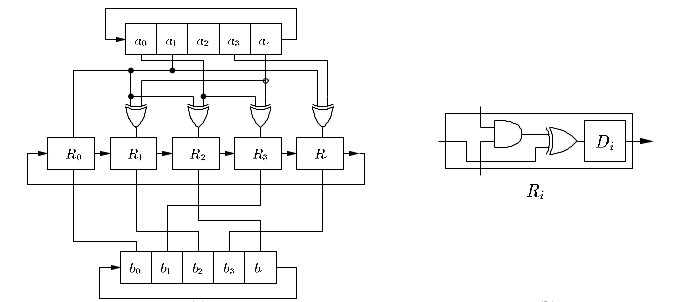
\includegraphics[scale=0.3]{./SMPO.png}}
    \caption{5-bit SMPO}
  \label{fig:SMPO}
  \end{figure}

Similarly, build elimination ideal for all gates/operations and induce
initial states of latches. However, instead of eliminating all variables
to one, this example adopts abstraction term order from \ref{thm:abs}
and keeps the polynomial contains function between output and inputs.
Here the lex ordering is $\{others\} > R > \{A, B\}$, and objective
polynimial is $R + \F(A, B)$. \par

Apply this approach to calculate image in BFS traversal, but modify 
\ref{alg:BFS} to make it adapt 6 steps reachable states enumeration.
The result is $R + AB$, which validates the function of this circuit.

\end{Example}
